\def\QRCODE{MASTER_mispa_TUT.IMG.morphological_geodesic_filtering_matlabqrcode.png}
\def\QRPAGE{http://www.iptutorials.science/tree/master/MASTER_mispa/TUT.IMG.morphological_geodesic_filtering/matlab}
\mcorrectionsection{Matlab correction}

\subsection{Morphological center}
The noisy image is obtained with the function \minline{imnoise}.
\begin{matlab}
A=double(imread('lena512.bmp'));
A=255*imnoise(A/255,'salt & pepper', 0.04);
\end{matlab}

Following the definition, the morphological center is obtained with the following code, and illustrated in Fig.\ref{fig:geodesic_filtering:matlab:center}:
\begin{matlab}
n=1;
se=strel('disk',n);
coc=imclose(imopen(imclose(A,se),se),se);
oco=imopen(imclose(imopen(A,se),se),se);
cMin=min(oco,coc);
cMax=max(oco,coc);
B=min(max(A,cMin),cMax);
\end{matlab}

\begin{figure}[htbp]
 \centering
%  \subfloat[Original image.]{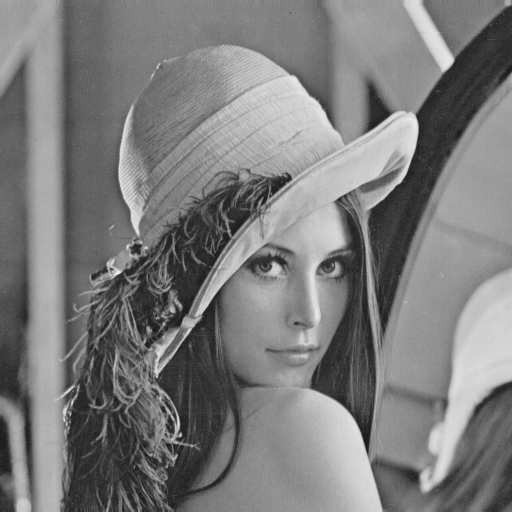
\includegraphics[width=.3\linewidth]{lena512.png}}
%  \hspace{1cm}
 \subfloat[Noisy image.]{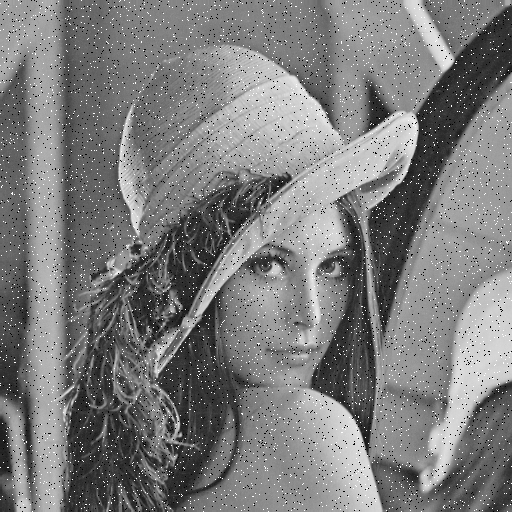
\includegraphics[width=.3\linewidth]{lena_noisy.png}}
 \hfill
 \subfloat[Median filter of size $5\times 5$.]{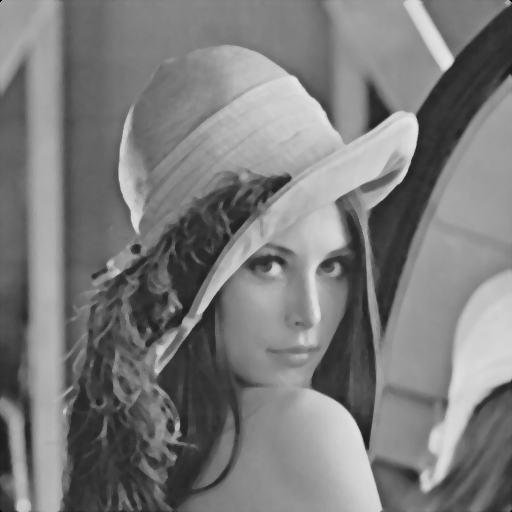
\includegraphics[width=.3\linewidth]{lena_median.png}}
 \hfill
 \subfloat[Morphological center.]{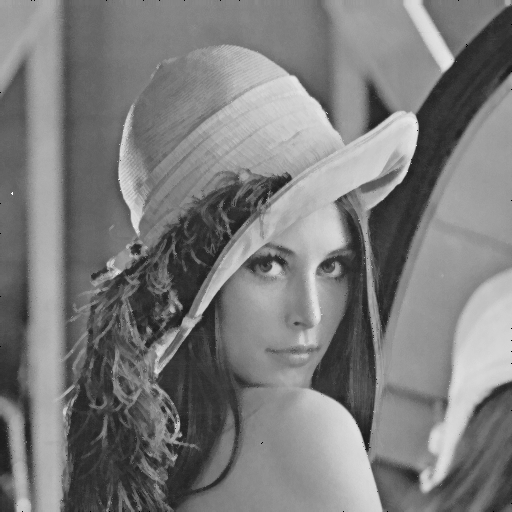
\includegraphics[width=.3\linewidth]{lena_center.png}}
 \caption{Morphological center compared to the classical median filter.}
 \label{fig:geodesic_filtering:matlab:center}
\end{figure}


\subsection{Alternate sequential filters}
The order of these filters are often chosen empirically. The results are illustrated in Fig.\ref{fig:geodesic_filtering:matlab:asf}.

\begin{matlab}
function F = asf_n(I, order)
% Alternate Sequential Filter beginning by a closing
% I: original image
% order: order of the filter (number of loops)
F = I;
for i=1:order
    se = strel('disk', i);
    F = imclose(imopen(F, se), se);
end
\end{matlab}

\begin{matlab}
function F = asf_m(I, order)
% Alternate Sequential Filter beginning by an opening
% I: original image
% order: order of the filter (number of loops)
F = I;
for i=1:order
    se = strel('disk', i);
    F = imopen(imclose(F, se), se);
end 
\end{matlab}

\begin{figure}[htbp]
 \centering
 \subfloat[Original image.]{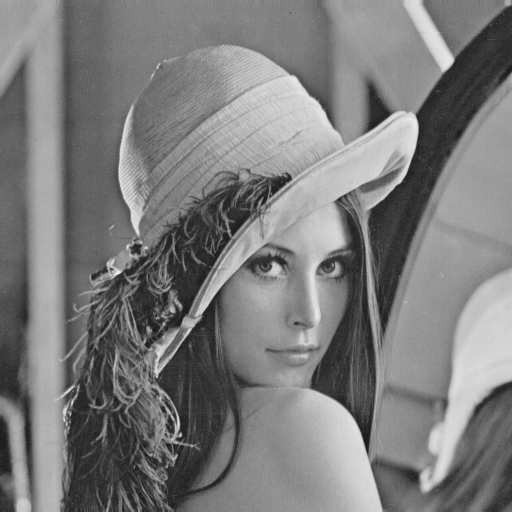
\includegraphics[width=.3\linewidth]{lena512.png}}
 \hfill
 \subfloat[ASF of order 3, starting with a closing operation (denoted N).]{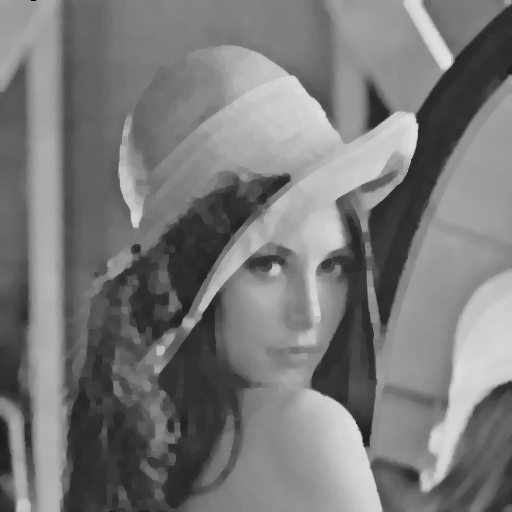
\includegraphics[width=.3\linewidth]{lena_asf_n.png}}
 \hfill
 \subfloat[ASF of order 3, starting with an opening operation (denoted M).]{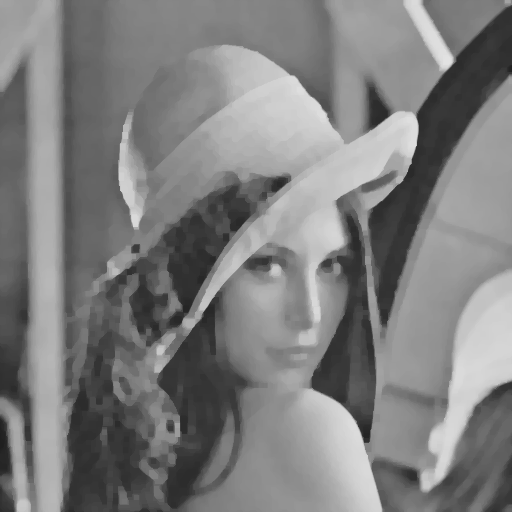
\includegraphics[width=.3\linewidth]{lena_asf_m.png}}
 \caption{Alternate Sequential Filters compared to original image.}
 \label{fig:geodesic_filtering:matlab:asf}
\end{figure}

\subsection{Geodesic reconstruction filters}
These two functions are simply implemented using erosion and reconstruction operators. Notice the duality property, that is used to code \minline{closerec}. In this example, 8 bits images (unsigned) are considered, and the results are illustrated in Fig.\ref{fig:geodesic_filtering:matlab:georec}.

\begin{matlab}
function D=openrec(A,n)
B=imerode(A,strel('disk',n));
D=reconstruct(A,B);
\end{matlab}

\begin{matlab}
function D=closerec(A,n)
% closerec and openrec are dual operators
D = 255-openrec(255-A, n); 
\end{matlab}

\begin{figure}[htbp]
 \centering
 \subfloat[Original image.]{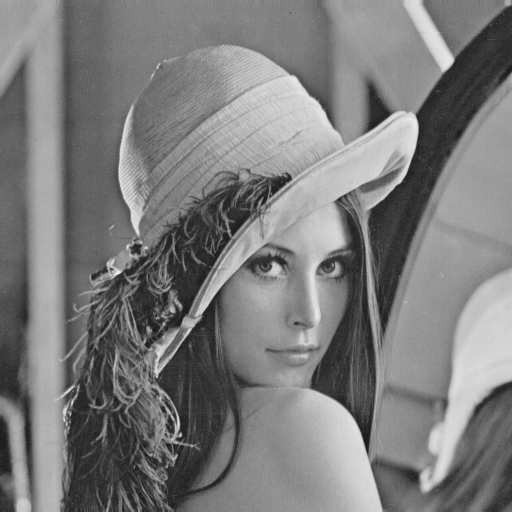
\includegraphics[width=.3\linewidth]{lena512.png}}
 \hfill
 \subfloat[Opening by reconstruction.]{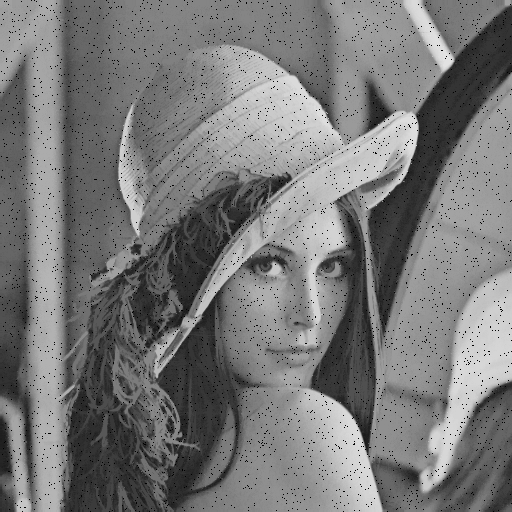
\includegraphics[width=.3\linewidth]{lena_openrec.png}}
 \hfill
 \subfloat[Closing by reconstruction.]{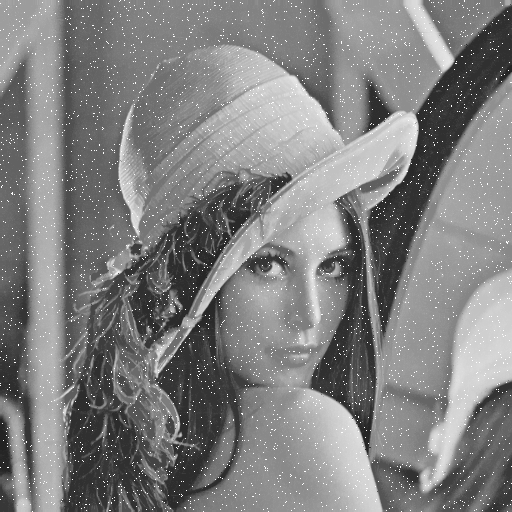
\includegraphics[width=.3\linewidth]{lena_closerec.png}}
 \caption{Opening and closing by reconstruction.}
 \label{fig:geodesic_filtering:matlab:georec}
\end{figure}

\subsection{ASF by reconstruction}
This is an example of a 3rd order alternate sequential filter, illustrated in Fig.\ref{fig:geodesic_filtering:matlab:asf_rec}.

\begin{matlab}
n1=1;
n2=2;
n3=3;
co1=closerec(openrec(A,n1),n1);
co2=closerec(openrec(co1,n2),n2);
co3=closerec(openrec(co2,n3),n3);
\end{matlab}

\begin{figure}[htbp]
 \centering
 \subfloat[Original image.]{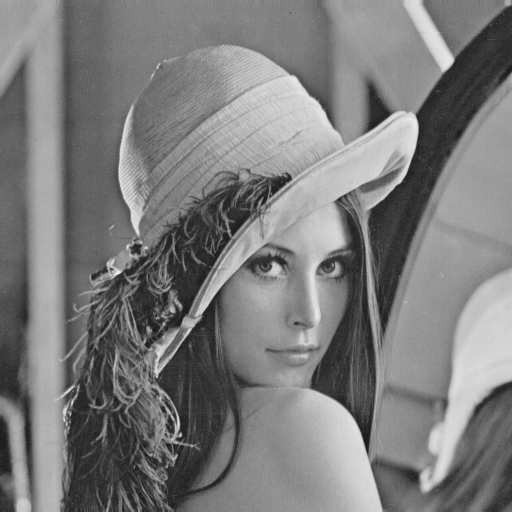
\includegraphics[width=.3\linewidth]{lena512.png}}
 \hfill
 \subfloat[ASF by reconstruction.]{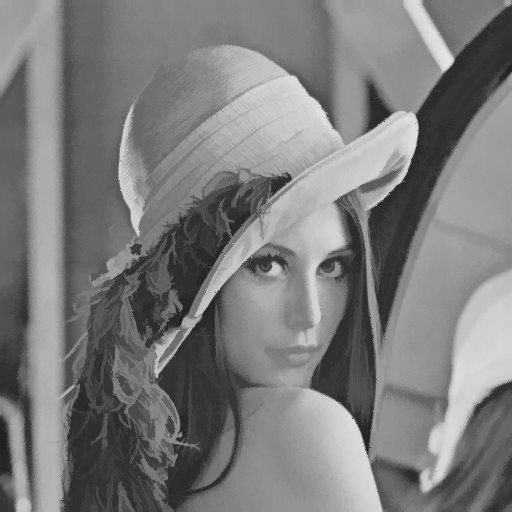
\includegraphics[width=.3\linewidth]{lena_asf_rec.png}}
 \hfill
 \subfloat[Noisy image.]{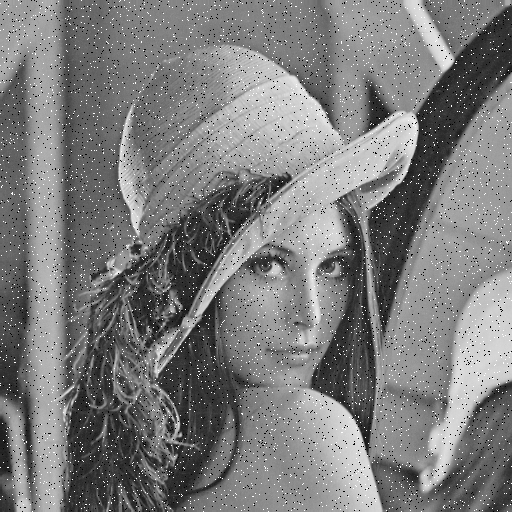
\includegraphics[width=.3\linewidth]{lena_noisy.png}}
 
 \caption{Alternate Sequential Filtering by reconstruction.}
 \label{fig:geodesic_filtering:matlab:asf_rec}
\end{figure}

\subsection{Morphological center by reconstruction}
Morphological center by reconstruction replaces the opening and closing operations by their equivalent by reconstruction (see Fig.\ref{fig:geodesic_filtering:matlab:center_rec}).

\begin{matlab}
n=1;
coc=closerec(openrec(closerec(A,n),n),n);
oco=openrec(closerec(openrec(A,n),n),n);
cMin=min(oco,coc);
cMax=max(oco,coc);
B=min(max(A,cMin),cMax);
\end{matlab}

\begin{figure}[htbp]
 \centering
 \subfloat[Original image.]{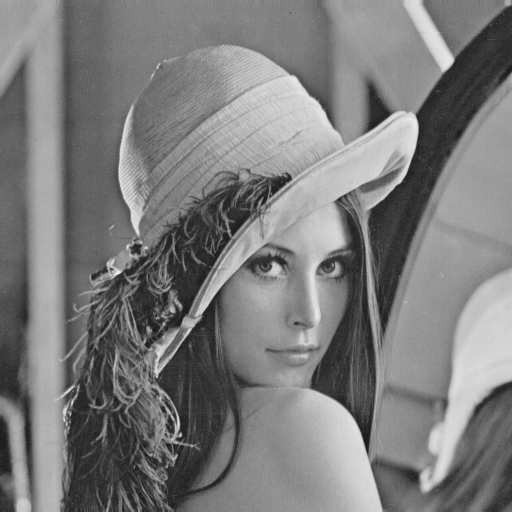
\includegraphics[width=.3\linewidth]{lena512.png}}
 \hfill
 \subfloat[Center by reconstruction.]{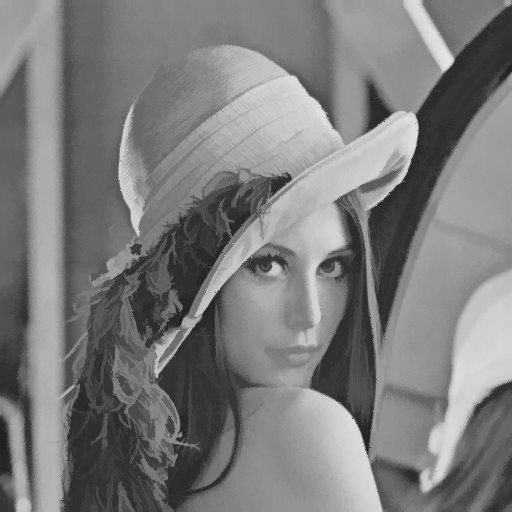
\includegraphics[width=.3\linewidth]{lena_center_rec.png}}
 \hfill
 \subfloat[Noisy image.]{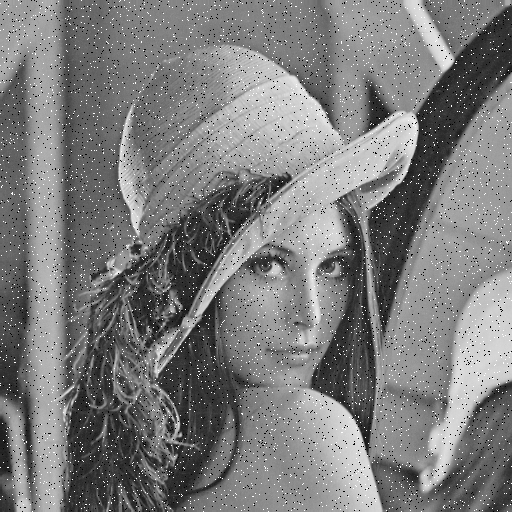
\includegraphics[width=.3\linewidth]{lena_noisy.png}}
 
 \caption{Morphological center by reconstruction.}
 \label{fig:geodesic_filtering:matlab:center_rec}
\end{figure}